\chapter{Implementation Overview}
\label{sec:implementation-overview}

The goal is to develop a secure Password Manager, where passwords are stored in a secure and removable USB device, that is based on SECube. Different challenges needs to be solved in order to achive this goal: from the SECube's firmware to the development of a Chromium Extension. \bigskip

The main problem is the communication between the Chromium Browser and the SECube: due to the high level of restrictions imposed by any modern web browser, indeed they act as a big and complex sandboxes for good reasons, it's nearly impossible to have a direct connection between the Extension and any physical device connected to the Host PC. \bigskip

Because of this, a third actor needs to be introduced: a middleware that is capable of being both interfaced with any (Chromium-based) browser and able to communicate with the SECube device. Thus, the middleware is a third software that is intended to be installed and run on the host PC continuosly (like a service on Windows or a deamon on Linux, or executed by the user when he needs it, as he prefers). \bigskip

\section{The solution}

\begin{figure}[H]
	\centering
	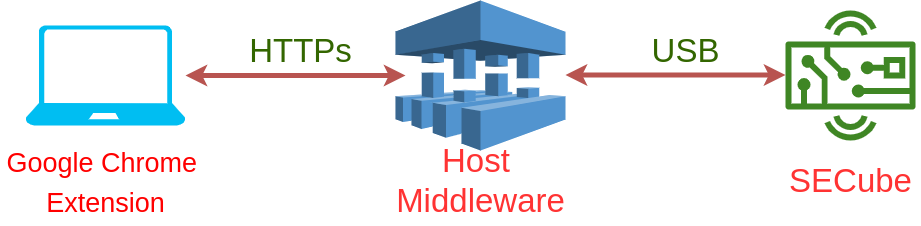
\includegraphics[width=0.9\linewidth]{images/overview}
	\caption{How the three actors interact between each other}
	\label{fig:overview}
\end{figure}

Due to all these actors, developing a secure Password Manager becomes very complicated. It is very important, in cases like this, to be pretty organized and try to be sistematic in developing all the needed software, without trying to reinvent the wheel. \bigskip

The three components have been developed completely indipendent from others one, trying to move all the possible logic and sensitive data to the lowest level (i.e. the Host Middleware and the SECube): this is due to the fact that these two actors are the most secure while the Extension is the most exposed one to possible threats. \bigskip

The communication between the Extenson and the Middleware happens by means of HTTPs: it is a secure version of HTTP based on TLS, allowing to have a complete communication between the two parties. The communication between the Middleware and the SECube happens by means of a USB connection, and the communication is encrypted. 

% In this chapter you should provide a general overview of the project, explaining what you have implemented staying at a high-level of abstraction, without going too much into the details. Leave details for the implementation chapter. This chapter can be organized in sections, such as goal of the project, issues to be solved, solution overview, etc.\\It is very important to add images, schemes, graphs to explain the original problem and your solution. Pictures are extremely useful to understand complex ideas that might need an entire page to be explained.\\Use multiple sections to explain the starting point of your project, the last section is going to be the high-level view of your solution...so take the reader in a short `journey` to showcase your work.